\section{Optical Emitting Payload}
	\label{blDOLSR}
		\subsection{Introduction}
Satellite altimetry missions use active remote sensing techniques. For that reason the quality of the system is dependent on the emitted electromagnetic radiation and the analysis of the returned signal. Considering the orbit of a regular Earth observation satellite to be in the order of 500 to 800 kilometers (statement based of earlier altimetry missions) and the fact that the power of the emitted radiation decreases exponentially with distance, finding a proper optical emitting device is not a simple task. Next to the decrease in energy, atmospheric absorption or scattering at specific wavelengths are also another important issues to consider, since altimetry missions usually are designed to measure the actual Earth's surface, i.e. the emitted photons need to be able to reach the surface, have enough energy to scatter and reach the receiver.

To be able to select any optical emitting device, the important parameters for optimizing the altimetry results should be revised. Several problems occur if emitting radiation is chosen as the remote sensing technique. 
\begin{enumerate}[i]
	\item First of all, general electromagnetic radiation will show isotropic behavior. This results in an effective energy loss, since most of the radiation is not pointed towards the desired position. Hence, a divergence limited source would be preferable.
	\item As mentioned before, the wavelength is an important parameter since it will influence the photons actually reaching Earth. Since the Earth's atmosphere is transparent for wavelengths in the visible spectrum, it would be better to have an electromagnetic radiation source with a wavelength in this interval. Next to that, a regular radiation source (like the Sun) emits radiation consisting of a whole spectrum of wavelengths. The less the number of discrete wavelengths (preferable in the visible spectrum), the higher the quality of the analysis can be.
	\item The total work done on the photons to reach the Earth's surface, scatter and return to the receiver, is generally very large. To cope with this large work, the energy of the specific energy pulses should be high.  
\end{enumerate}

All of these criteria are important when considering the optical emitting device. The most convenient mechanism for solving these preliminary problems can be solved by using a \ac{laser} system. Optical emitting devices using \acs{laser} technique have considerably low divergence (high energy density),  discrete and known wavelength characteristics and a relative high pulse energy.

\subsection{Laser Characteristics}
	\label{blDOLSRchar}
The characteristics of \acs{laser} systems are determined by the quantum mechanical interaction of electrons (and holes) between the conduction and valence band. Quantum mechanics predicts that electron energy levels are discrete and quantizised, hence, predicting the existences of energy gaps. The electron configuration in a given chemical element,will be distributed according to the Boltzmann distribution, assuming the element is in thermal equilibrium. Generally, the electrons will exhibit the lowest energy state. Electron excitation can take place by energy addition to an $n$-level energy system, where $n$ denotes the number of quantizised energy levels. This energy can be thermal, electric or photonic. 

Photonic excitation, i.e. electron excitation by an induced photon, can lead to stimulated emission, which is the starting point for the working principle of the \acs{laser} technique. To achieve photonic excitation, the energy of the incoming photon should be equal to the the difference in electron energy level from ground state to excited state. Since this energy is dependent on wavelength, the resulting wavelength of the \acs{laser} radiation is known as well (incoming wavelength equals wavelength laser radiation). Every chemical composition has its characteristic discrete energy levels and bandgaps, allowing different bandgap energies and hence, different wavelength characteristics. 

The \acs{laser} is an optical emitting device consisting of a certain aperture value. For this reason, diffraction will occur. However, due to the low divergence, the diffraction will be lower relative to isotropic radiating sources.

Radiation from the \acs{laser} can be continuous or pulsed. The input power, also known as the pump power, is the power needed to ensure the right amount of stimulated electron emission in the \acs{laser} cavity. This power is then redirected towards the radiation. Since many \acs{laser}s are pulsed, with pulses in the order of pico- to nanoseconds with relatively high frequency, the pulse power, i.e. the power divided per unit pulse, is in the order of 0.001 to 1 Watt. Peak powers in that case can exceed 1 gigawatt \cite{quantumoptics}.  

\subsection{Laser Types}
	\label{blDOLSRtypes}
There are actually many types of \acs{laser}s. The main types are considered below:
\begin{enumerate}
	\item Gas. A variety of \acs{laser}s is based on gases as gain media. The \acs{laser}-active entities are either single atoms or molecules, and are often used in a mixture with other substances having auxiliary functions. Most gas lasers emit with a high beam quality, often close to diffraction-limit, since the gas introduces only weak optical distortions.
	\item Semiconductor \acs{laser}s, also known as diode \acs{laser}s, are \acs{laser}s based on semiconductor gain media, where the optical gain is usually achieved by stimulated emission at an interband transition under conditions of a high carrier density in the conduction band.  
	\item Solid-State \acs{laser}s are \acs{laser}s based on solid-state gain media such as crystals or glasses doped with rare Earth or transition metal ions. They are mainly optically pumped with flash lamps or arc lamps, which will lead to high powers and low costs but also to relative low power efficiencies and moderate lifetime. \cite{lasertech}
\end{enumerate} 
Figure \ref{DOS_laser} on page \pageref{DOS_laser} gives the final design option tree of the laser emitter.

\begin{figure} [!ht]
	\centering
	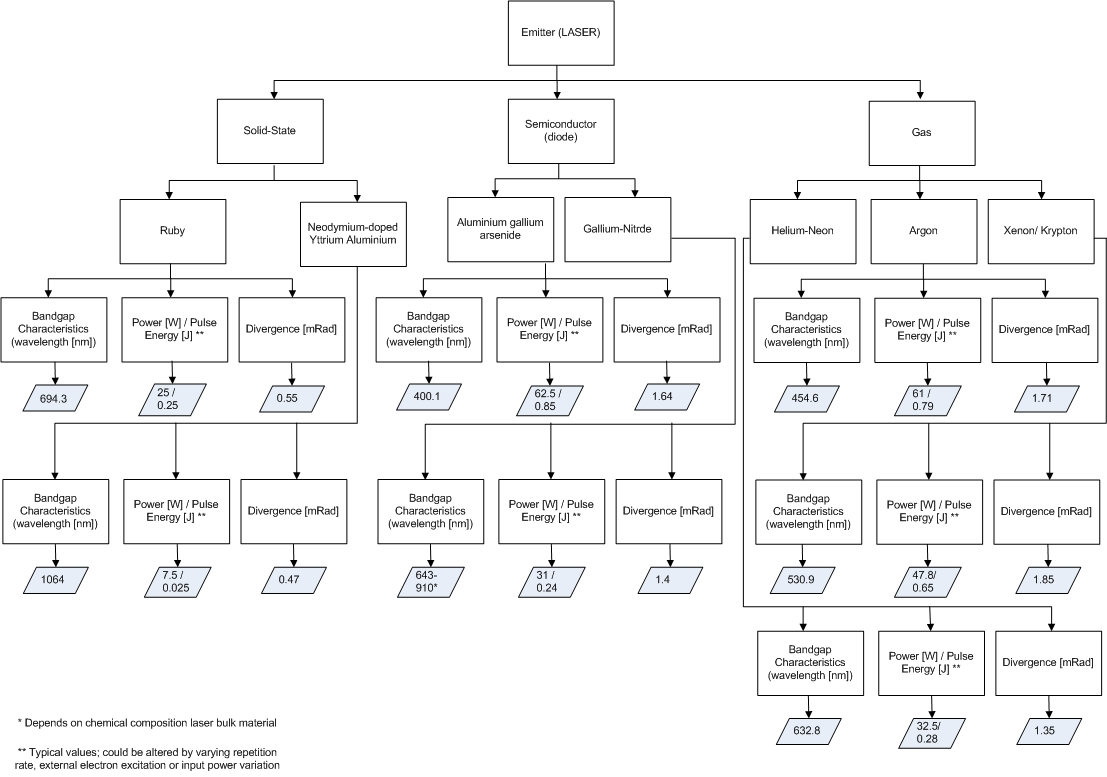
\includegraphics[height=0.85\textwidth,angle=90]{chapters/img/DOStree_laser.jpg}	
	\caption{Design option tree of laser emitter. Numbers indicate typical values.}
	\label{DOS_laser}
\end{figure}